% Prof. Dr. Ausberto S. Castro Vera
% UENF - CCT - LCMAT - Curso de Ci\^{e}ncia da Computa\c{c}\~{a}o
% Campos, RJ,  2022
% Disciplina: An\'{a}lise e Projeto de Sistemas
% Aluno:


\chapterimage{sistemas.png} % Table of contents heading image
\chapter{ Introdu\c{c}\~{a}o}

O \textit{Sistema remoto de gerenciamento de Carros Autônomos} tem como objetivo buscar uma descentralização de veículos autônomos, de modo que os veículos circulem por todos os 27 estados do Brasil conectados através de torres de comunicação 5G.
A empresa propõe que seus veículos percorrem as cidades do país 24 horas por dia, transportando passageiros que solicitarem carona pelo aplicativo. Após a conclusão bem-sucedida dessas solicitações, o veículo mais próximo se dirigirá ao passageiro.
Esses mesmos veículos da empresa só são desligados quando há necessidade de manutenção, medidas de precaução e suprimentos. Este sistema é gerenciado remotamente por desenvolvedores e colaboradores sem a necessidade de colaboradores em um local central. Esses funcionários se comunicam por meio de um sistema interno projetado para manter a comunicação segura e rápida entre os funcionários.

Além disso, o desenvolvimento deste projeto também visa conectar os veículos da empresa. Esses veículos serão desenvolvidos por uma empresa terceirizada que já os projetam para receber o software de inteligência artificial desenvolvido desde o início pela empresa compradora desses carros. A conexão desses veículos funcionará a partir de torres de comunicação 5G que estão espalhadas por todo o Brasil e essas torres são conectadas a satélites espalhados por todo o planeta.

Dessa forma, o acesso a satélites de comunicação e recursos em nuvem é contratado por empresas terceirizadas.
É importante ressaltar que os recursos de projeto, desenvolvimento e manutenção desses veículos são provenientes de empresas terceirizadas.

Este projeto tem como foco a implantação desta tecnologia no Brasil. Aqui, entre outras coisas, são apresentados seus requisitos, recursos, casos de uso, componentes, orçamentos para viabilizar a realização deste sistema.



Neste primeiro capítulo de abertura descreve, e elabora o projeto a ser desenvolvido.



\section{Descri\c{c}\~{a}o do Sistema Computacional a desenvolver}
Esta seção apresenta informações sobre o sistema, prioridades e justificativas para atingir seus objetivos gerais de facilitar a comunicação entre os veículos da empresa, seus usuários, e facilitar as transações. A partir de um sistema que agiliza o processo de localização dos veículos da empresa e encaminha esses recursos para o usuário final.

%\textbf{Aplicativo}


\subsection{Aplicativo}

Um dos principais objetivos do projeto é oferecer aos usuários uma agilidade no processo de encaminhamento de veículos, onde possam ter uma boa experiência com um sistema mais inteligente.
Dessa forma é possível, por meio do aplicativo, solicitar o veículo mais próximo que atenda às necessidades do usuário, bem como planejar viagens, consultar viagens anteriores, dar feedback sobre o serviço prestado pela empresa e cadastrar uma forma de pagamento.


\subsection{Sistema de gerenciamento de recursos}

Sistema de comunicação interna dos colaboradores e gestão dos recursos da empresa; Os veículos. Desta forma, propõe-se o desenvolvimento de um sistema que permita esta integração, de forma a facilitar e agilizar os processos diários. Este sistema também visa proporcionar à empresa um ambiente de trabalho remoto pensado para manter a comunicação segura e rápida entre os colaboradores. Além disso, podem ser consultadas informações sobre os veículos da empresa, como tempo de uso, manutenção, viagens já realizadas, localizações, status, tanque atual, despesas, lucros.

\section{Identificando as componentes do meu sistema}

Esta seção identifica os componentes necessários para a operação e design do sistema, incluindo desde o hardware até o as necessidade de recursos em nuvem que serão essenciais para que o sistema atenda a sua proposta móvel.


\subsection{Componente: Hardware} \label{Hardware}
\begin{figure}[H]
       \begin{center}
              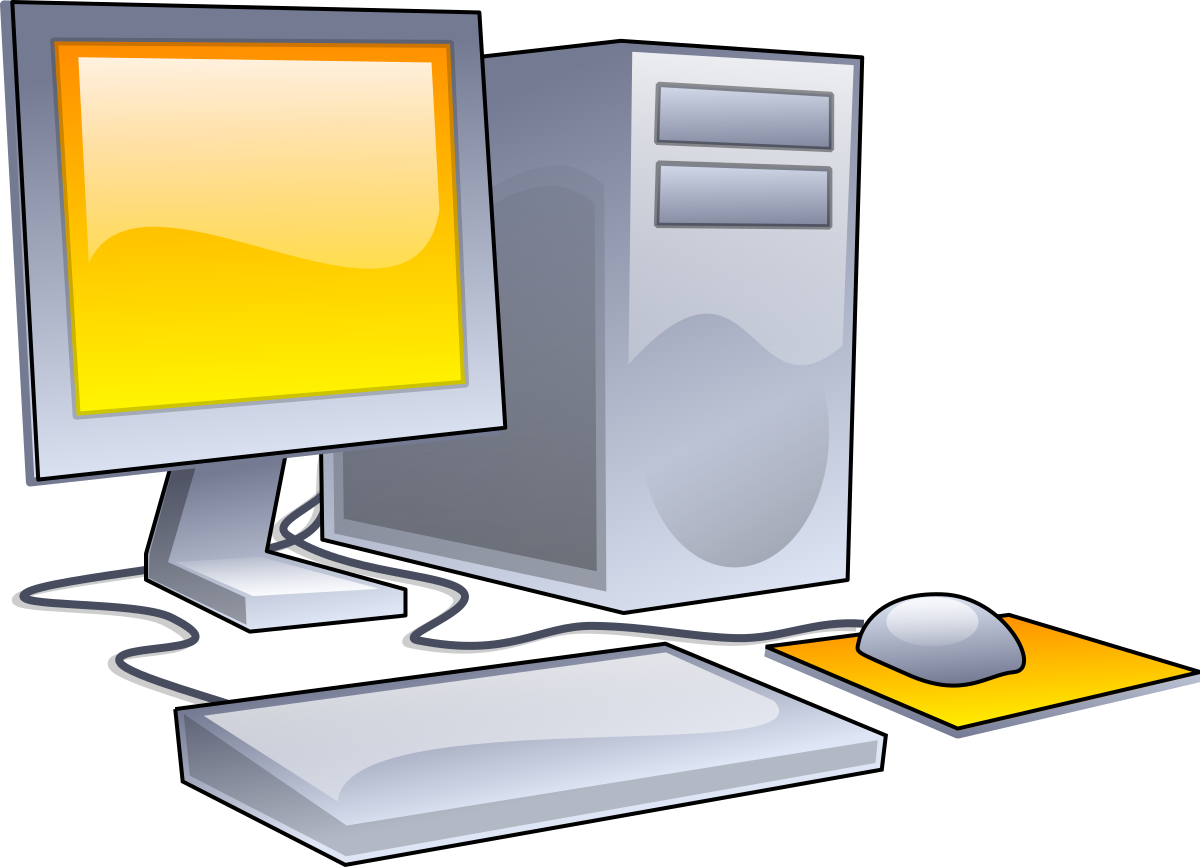
\includegraphics[width=8cm]{computer.png}
              \caption{Computador} \label{sistema}
       \end{center}
\end{figure}


\begin{itemize}


       \item \textbf{Workstation};
       \subitem Um (1) para cada funcionario em modalidade remota.
       \item \textbf{Gerador de energia};
       \subitem Um (1) para cada torre de comunicação.
       \item \textbf{Carros};
       \subitem - Sensores externos;
       \subitem - Câmera estereoscópica;
       \subitem - Câmera infravermelha;
       \subitem - Radar;
       \subitem - Sonar;
       \subitem - LIDAR;
       \item \textbf{Torres de Comunicação 5g};

 %      \item Computadores;
 %      \item Nobreaks;
 %      \item Estabilizadores;
 %      \item Switchs;
 %      \item Roteadores;
 %      \item Servidores; Aplicativo, Dados.;
 %      \item Ar condicionado para a sala de servidores;
 %      \item Impressoras;
 %      \item Mobília.

\end{itemize}

\subsection{Componente: Software}
\begin{figure}[H]
       \begin{center}
              
\includegraphics[width=8cm]{windows.jpg}
              \caption{Windows} \label{sistema}
       \end{center}
\end{figure}

\begin{figure}[H]
       \begin{center}
              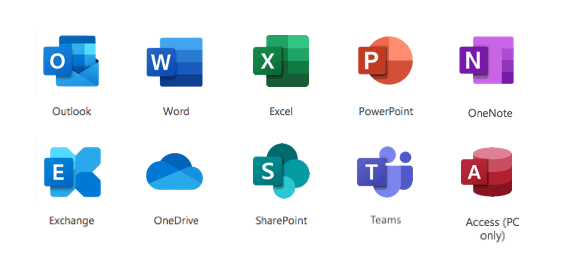
\includegraphics[width=8cm]{office.png}
              \caption{Pacote office} \label{sistema}
       \end{center}
\end{figure}

\begin{itemize}

       \item \textbf{Sistemas de controle};
       \subitem - ESC (Controle Eletrônico de Estabilidade)
       \subitem - iBooster
       \subitem - GPS, velocímetro e hodômetro
       \subitem - Inteligência Artificial e conectividade
       \item \textbf{Sistema;}
             \subitem - Sistema Administrativo.
             \subsubitem - Gerenciamento de Finanças.
             \subitem - Sistema de Gestão de recursos.
             \subitem - Sistema de RH.
             \subsubitem - Gerenciamento de Funcionários.


       \item \textbf{Sistemas operacionais proprietário};
       \item \textbf{Sistema operacionais};
             \subitem - Windows, Android, IOS.
       \item \textbf{Pacotes Offie}.


\end{itemize}

\subsection{Componente: Pessoas}

\begin{figure}[H]
       \begin{center}
              
\includegraphics[width=8cm]{users.png}
              \caption{Usuarios} \label{sistema}
       \end{center}
\end{figure}

\begin{figure}[H]
       \begin{center}
              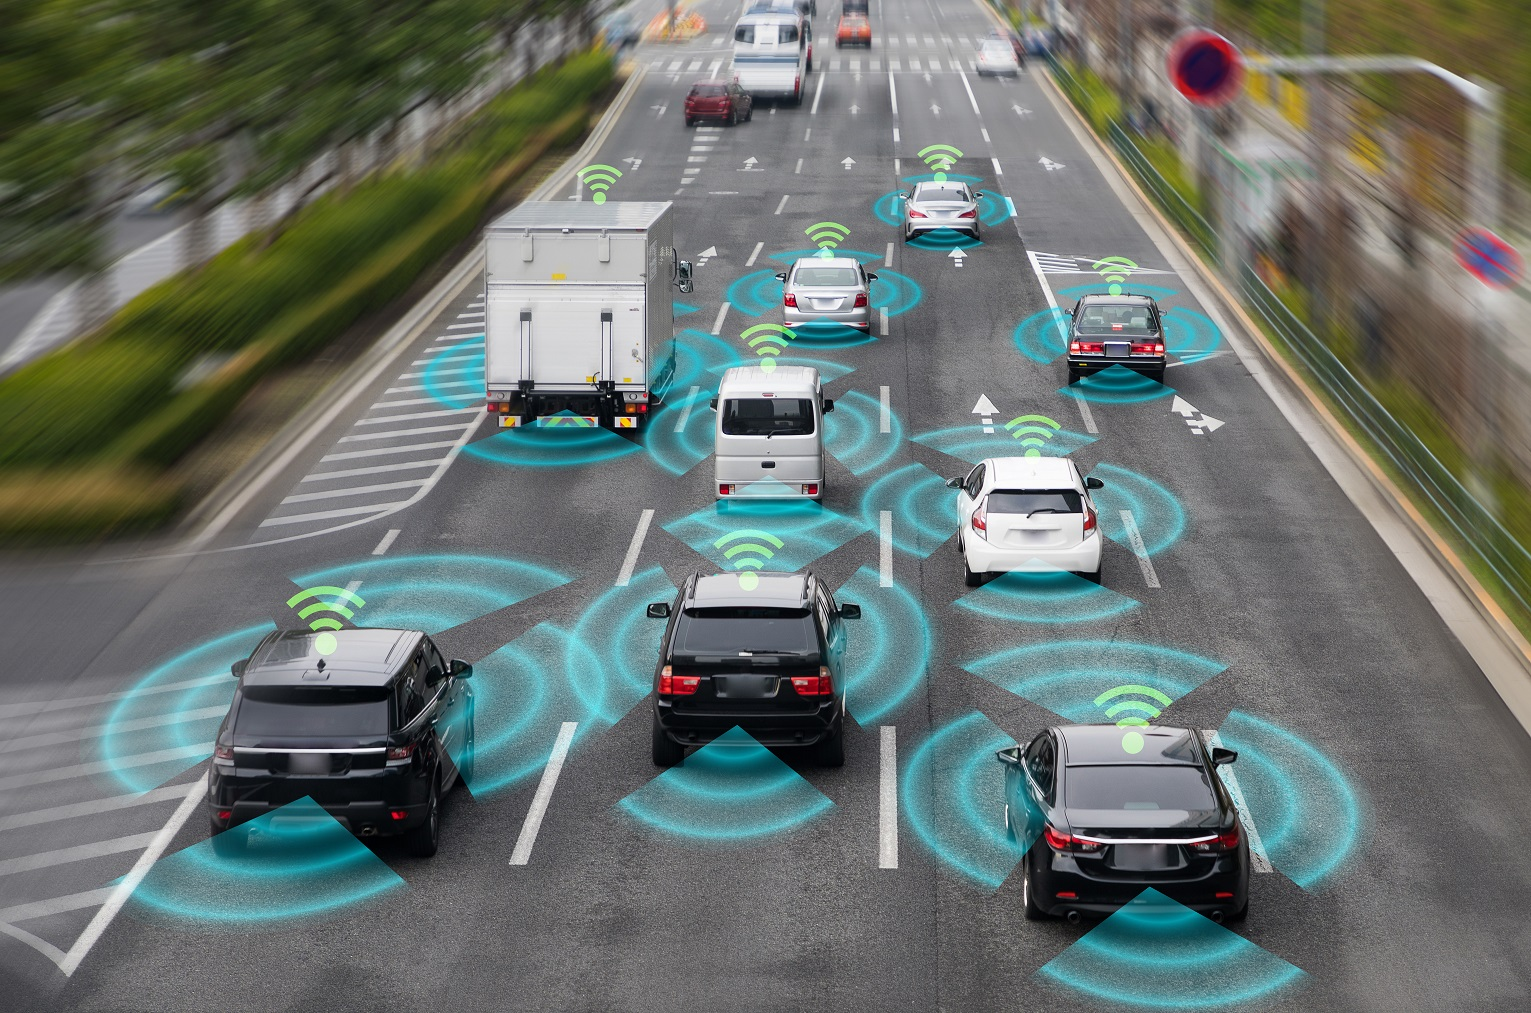
\includegraphics[width=8cm]{car_network.jpeg}
              \caption{Car Network} \label{sistema}
       \end{center}
\end{figure}
\begin{figure}[H]
       \begin{center}
              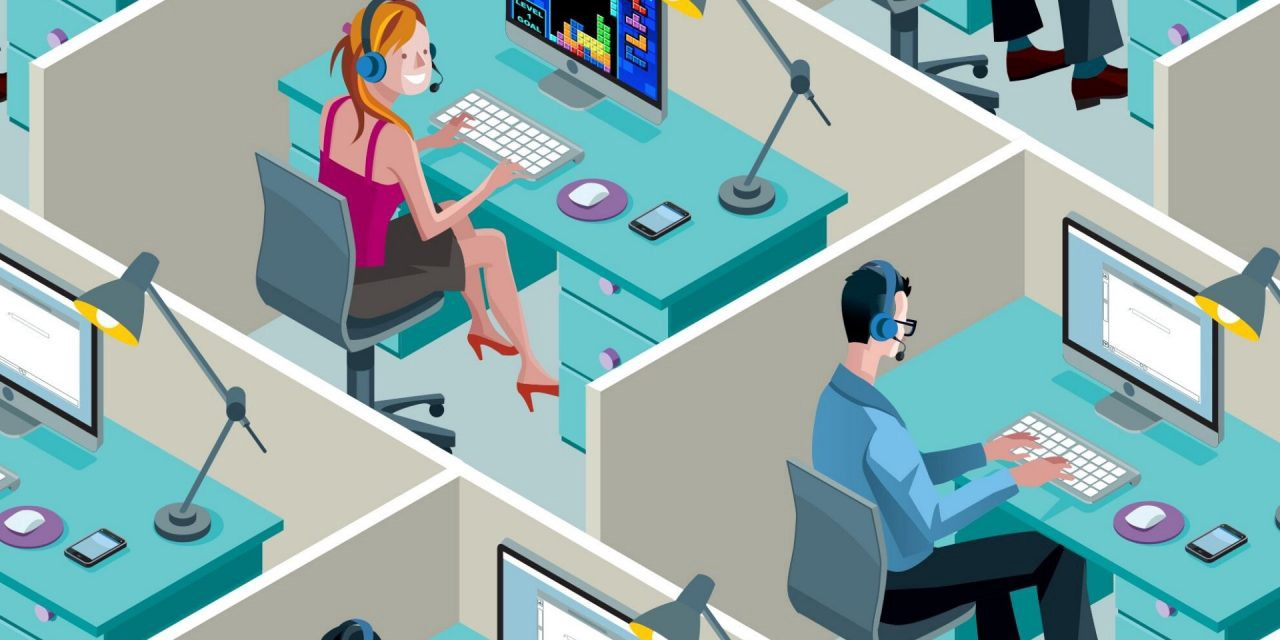
\includegraphics[width=8cm]{workers.jpg}
              \caption{Trabalhadores} \label{sistema}
       \end{center}
\end{figure}

\begin{itemize}

       \item Equipe de pesquisa;
       \item Engenheiro de Machine Learning;
       \item Equipe  de Inteligencia Artificial;
       \item Telecomunicação ;
       \item Analista de software;
       \item Gerente de projeto;
       \item Desenvolvedores;
       \item Técnicos de rede;
       \item Operador de banco de dados;
       \item Equipe de manutenção;
       \item Clientes;
       \item Programadores;
       \item Analista de Sistema;
       \item Chefe do Projeto;
       \item Arquitetos de software;
       \item Projetista;
       \item Avaliadores de Qualidade;
       \item   Funcionários  do RH;
       \item Funcionários de manutenção.

\end{itemize}
\subsection{Componente: Banco de Dados}

\begin{figure}[H]
       \begin{center}
              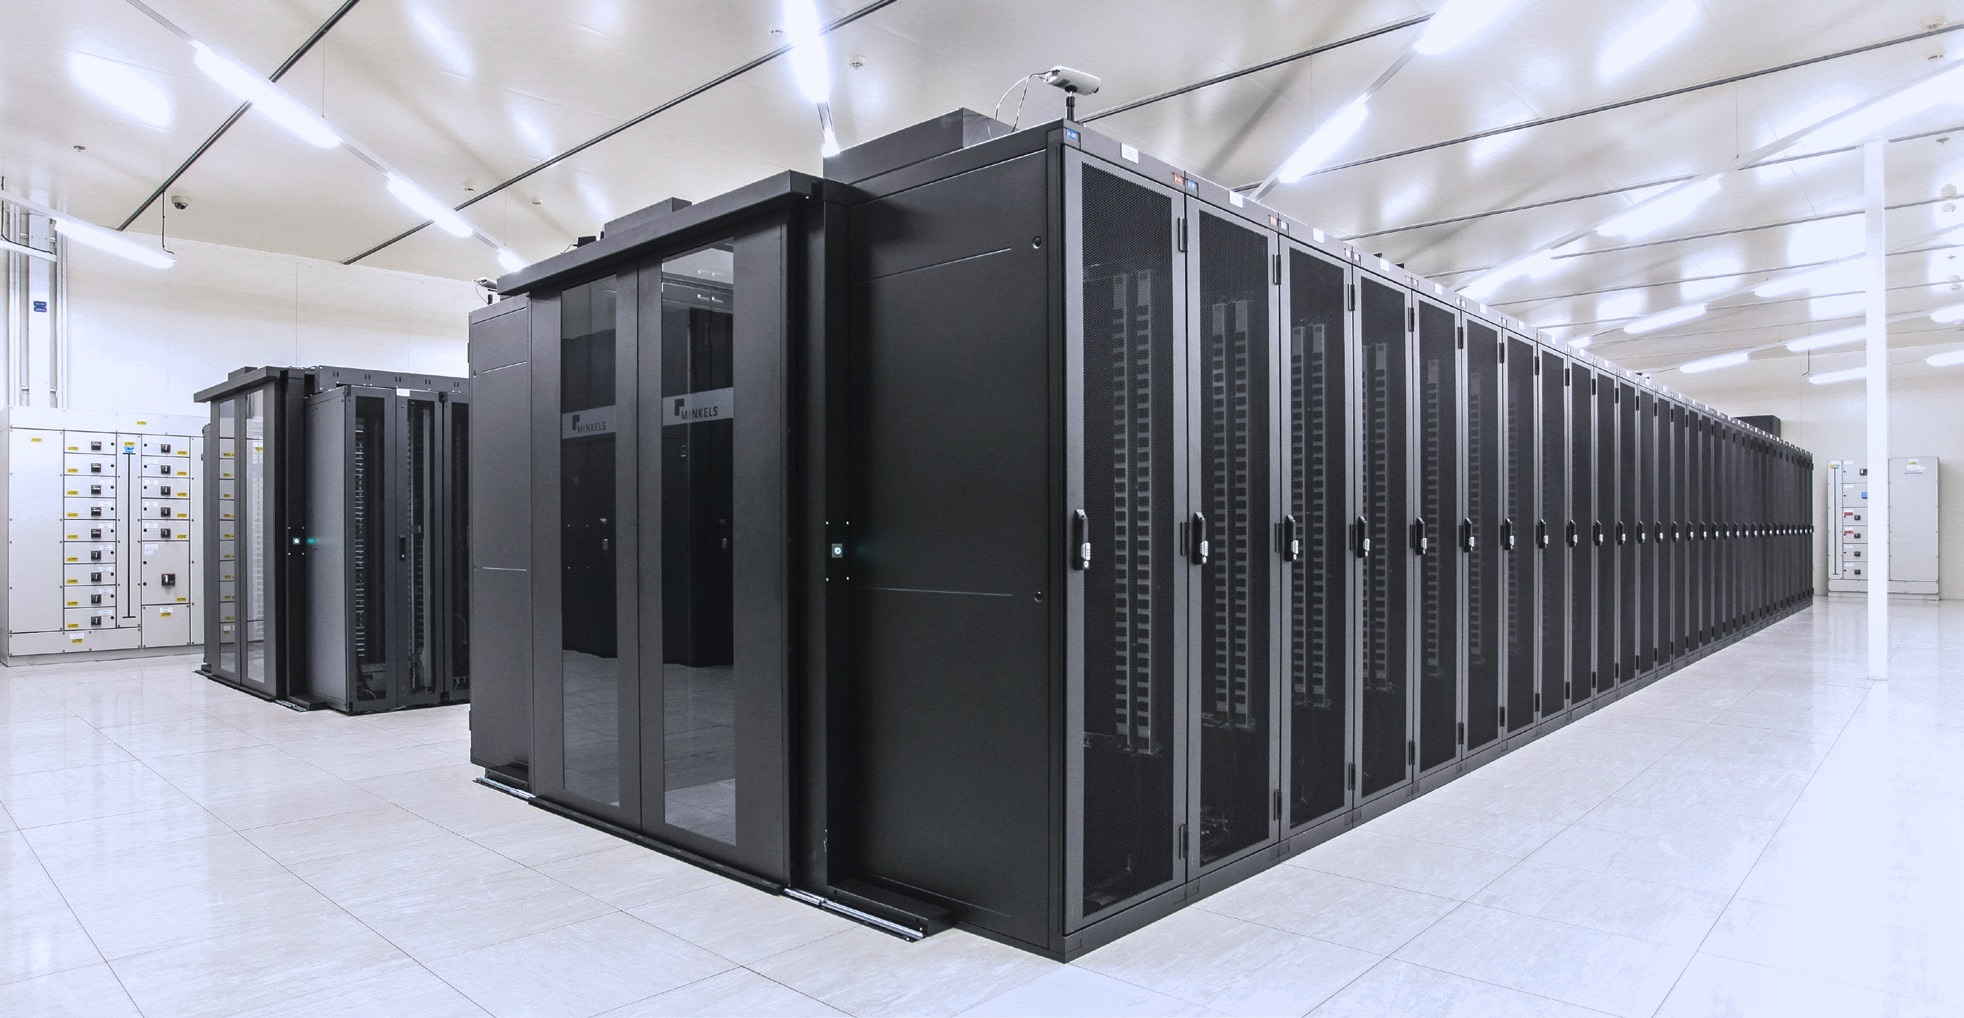
\includegraphics[width=8cm]{datacenter.jpg}
              \caption{Datacenter} \label{sistema}
       \end{center}
\end{figure}

\begin{figure}[H]
       \begin{center}
              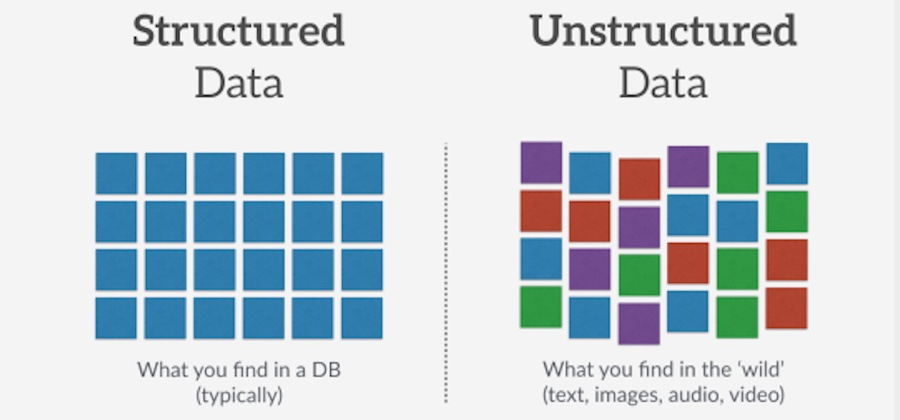
\includegraphics[width=8cm]{data.jpg}
              \caption{Tipos de dados} \label{sistema}
       \end{center}
\end{figure}

\begin{itemize}

       \item Veiculos;
       \item Receita;
       \item Funcionarios;
       \item Corridas realizadas.
       \end{itemize}

\subsection{Componente: Documentos }

\begin{figure}[H]
       \begin{center}
              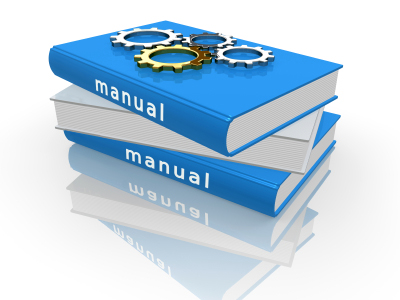
\includegraphics[width=8cm]{manuais.jpg}
              \caption{Manuais} \label{sistema}
       \end{center}
\end{figure}

\begin{figure}[H]
       \begin{center}
              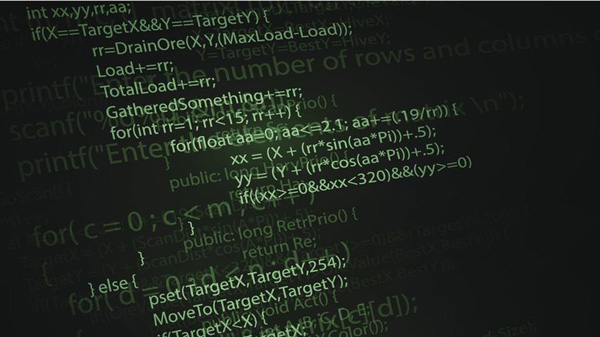
\includegraphics[width=8cm]{source-code.jpg}
              \caption{Códigos fonte} \label{sistema}
       \end{center}
\end{figure}

\begin{itemize}
       \item Confirmação de transações;
       \item Manuais do sistema;
       \item Diagramas UML;
       \item Relatórios;
       \item Orçamentos;
       \item Códigos fonte;
       \item Documentos comerciais;
       \item Manuais;
       \item Cronogramas.
     \end{itemize}

\subsection{Componente: Metodologias ou Procedimentos}

\begin{figure}[H]
       \begin{center}
              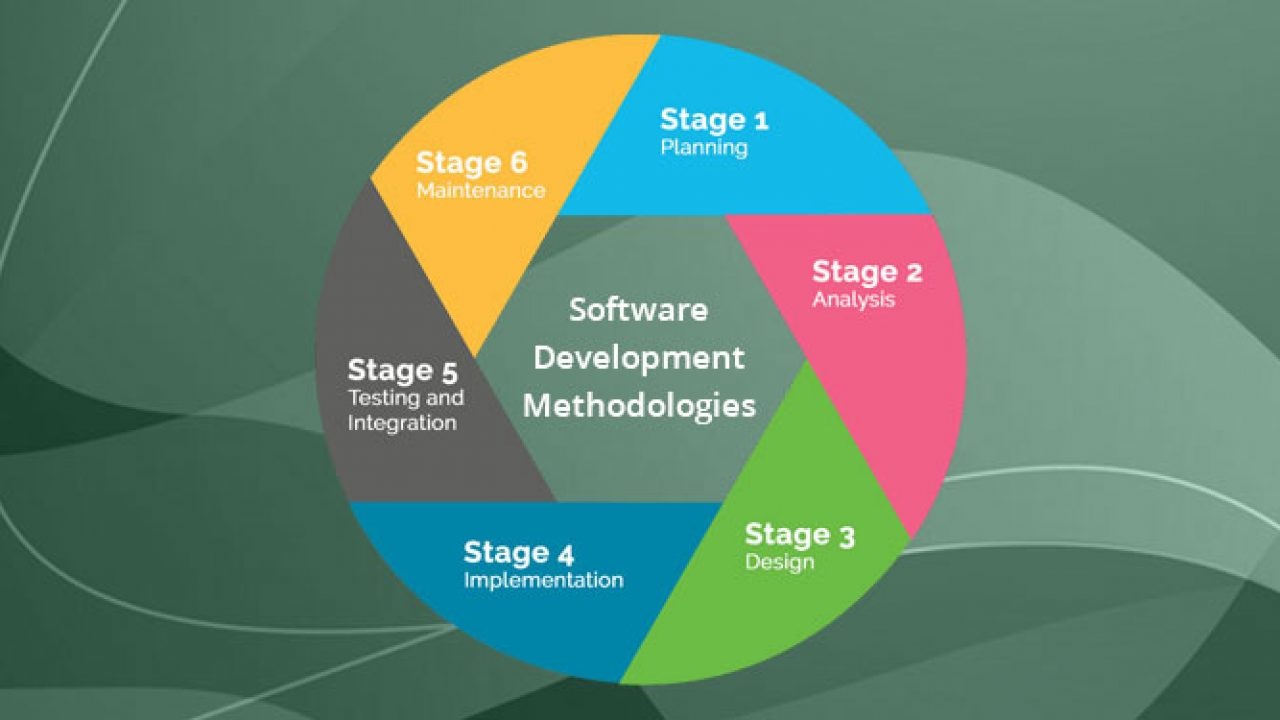
\includegraphics[width=8cm]{top-12-somethodologies.jpg}
              \caption{Metodologias} \label{sistema}
       \end{center}
\end{figure}

\begin{figure}[H]
       \begin{center}
              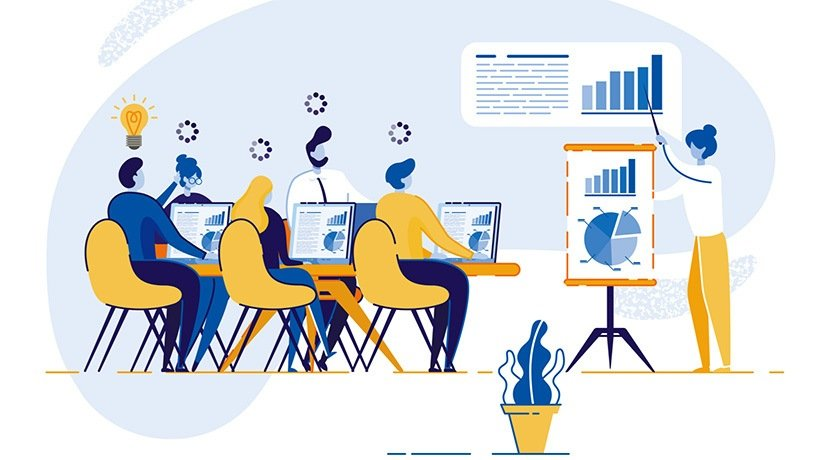
\includegraphics[width=8cm]{training.jpg}
              \caption{Trainamentos} \label{sistema}
       \end{center}
\end{figure}


\begin{itemize}
       \item \textbf{Levantamento de requisitos}
         \subitem - Relatório dos componentes do sistema;

        \item\textbf{ Analise}
         \subitem - Construção do modelo de representação do desenvolvimento do sistema;
          \subitem - Estudo da interação dos componentes com o sistema;
           \subitem  - Estudo detalhado dos requisitos;

         \item \textbf{Implementação}
          \subitem - Criação de aplicativo da empresa;
           \subitem  - Criação do Banco de Dados;
            \subitem - Montagem do servidor em nuvem;

          \item \textbf{Testes}
         \subitem - Teste para verificação de falhas no sistema;
          \subitem - Verificação de segurança;

           \item \textbf{Treinamento dos Funcionários para prestar suporte aos usuários}
         \subitem - O treinamento do suporte técnico;

          \item \textbf{Implantação}
         \subitem -Sistema colocado no Ambiente de usuário
          \subitem -Manual do sistema realizado
         \subitem -Realização da importação dos dados
          \subitem -A implantação do sistema deverá ser feita em gradualmente sem atrapalhar o funcionamento do hospital
         \end{itemize}

\subsection{Componente: Mobilidade}

\begin{figure}[H]
       \begin{center}
              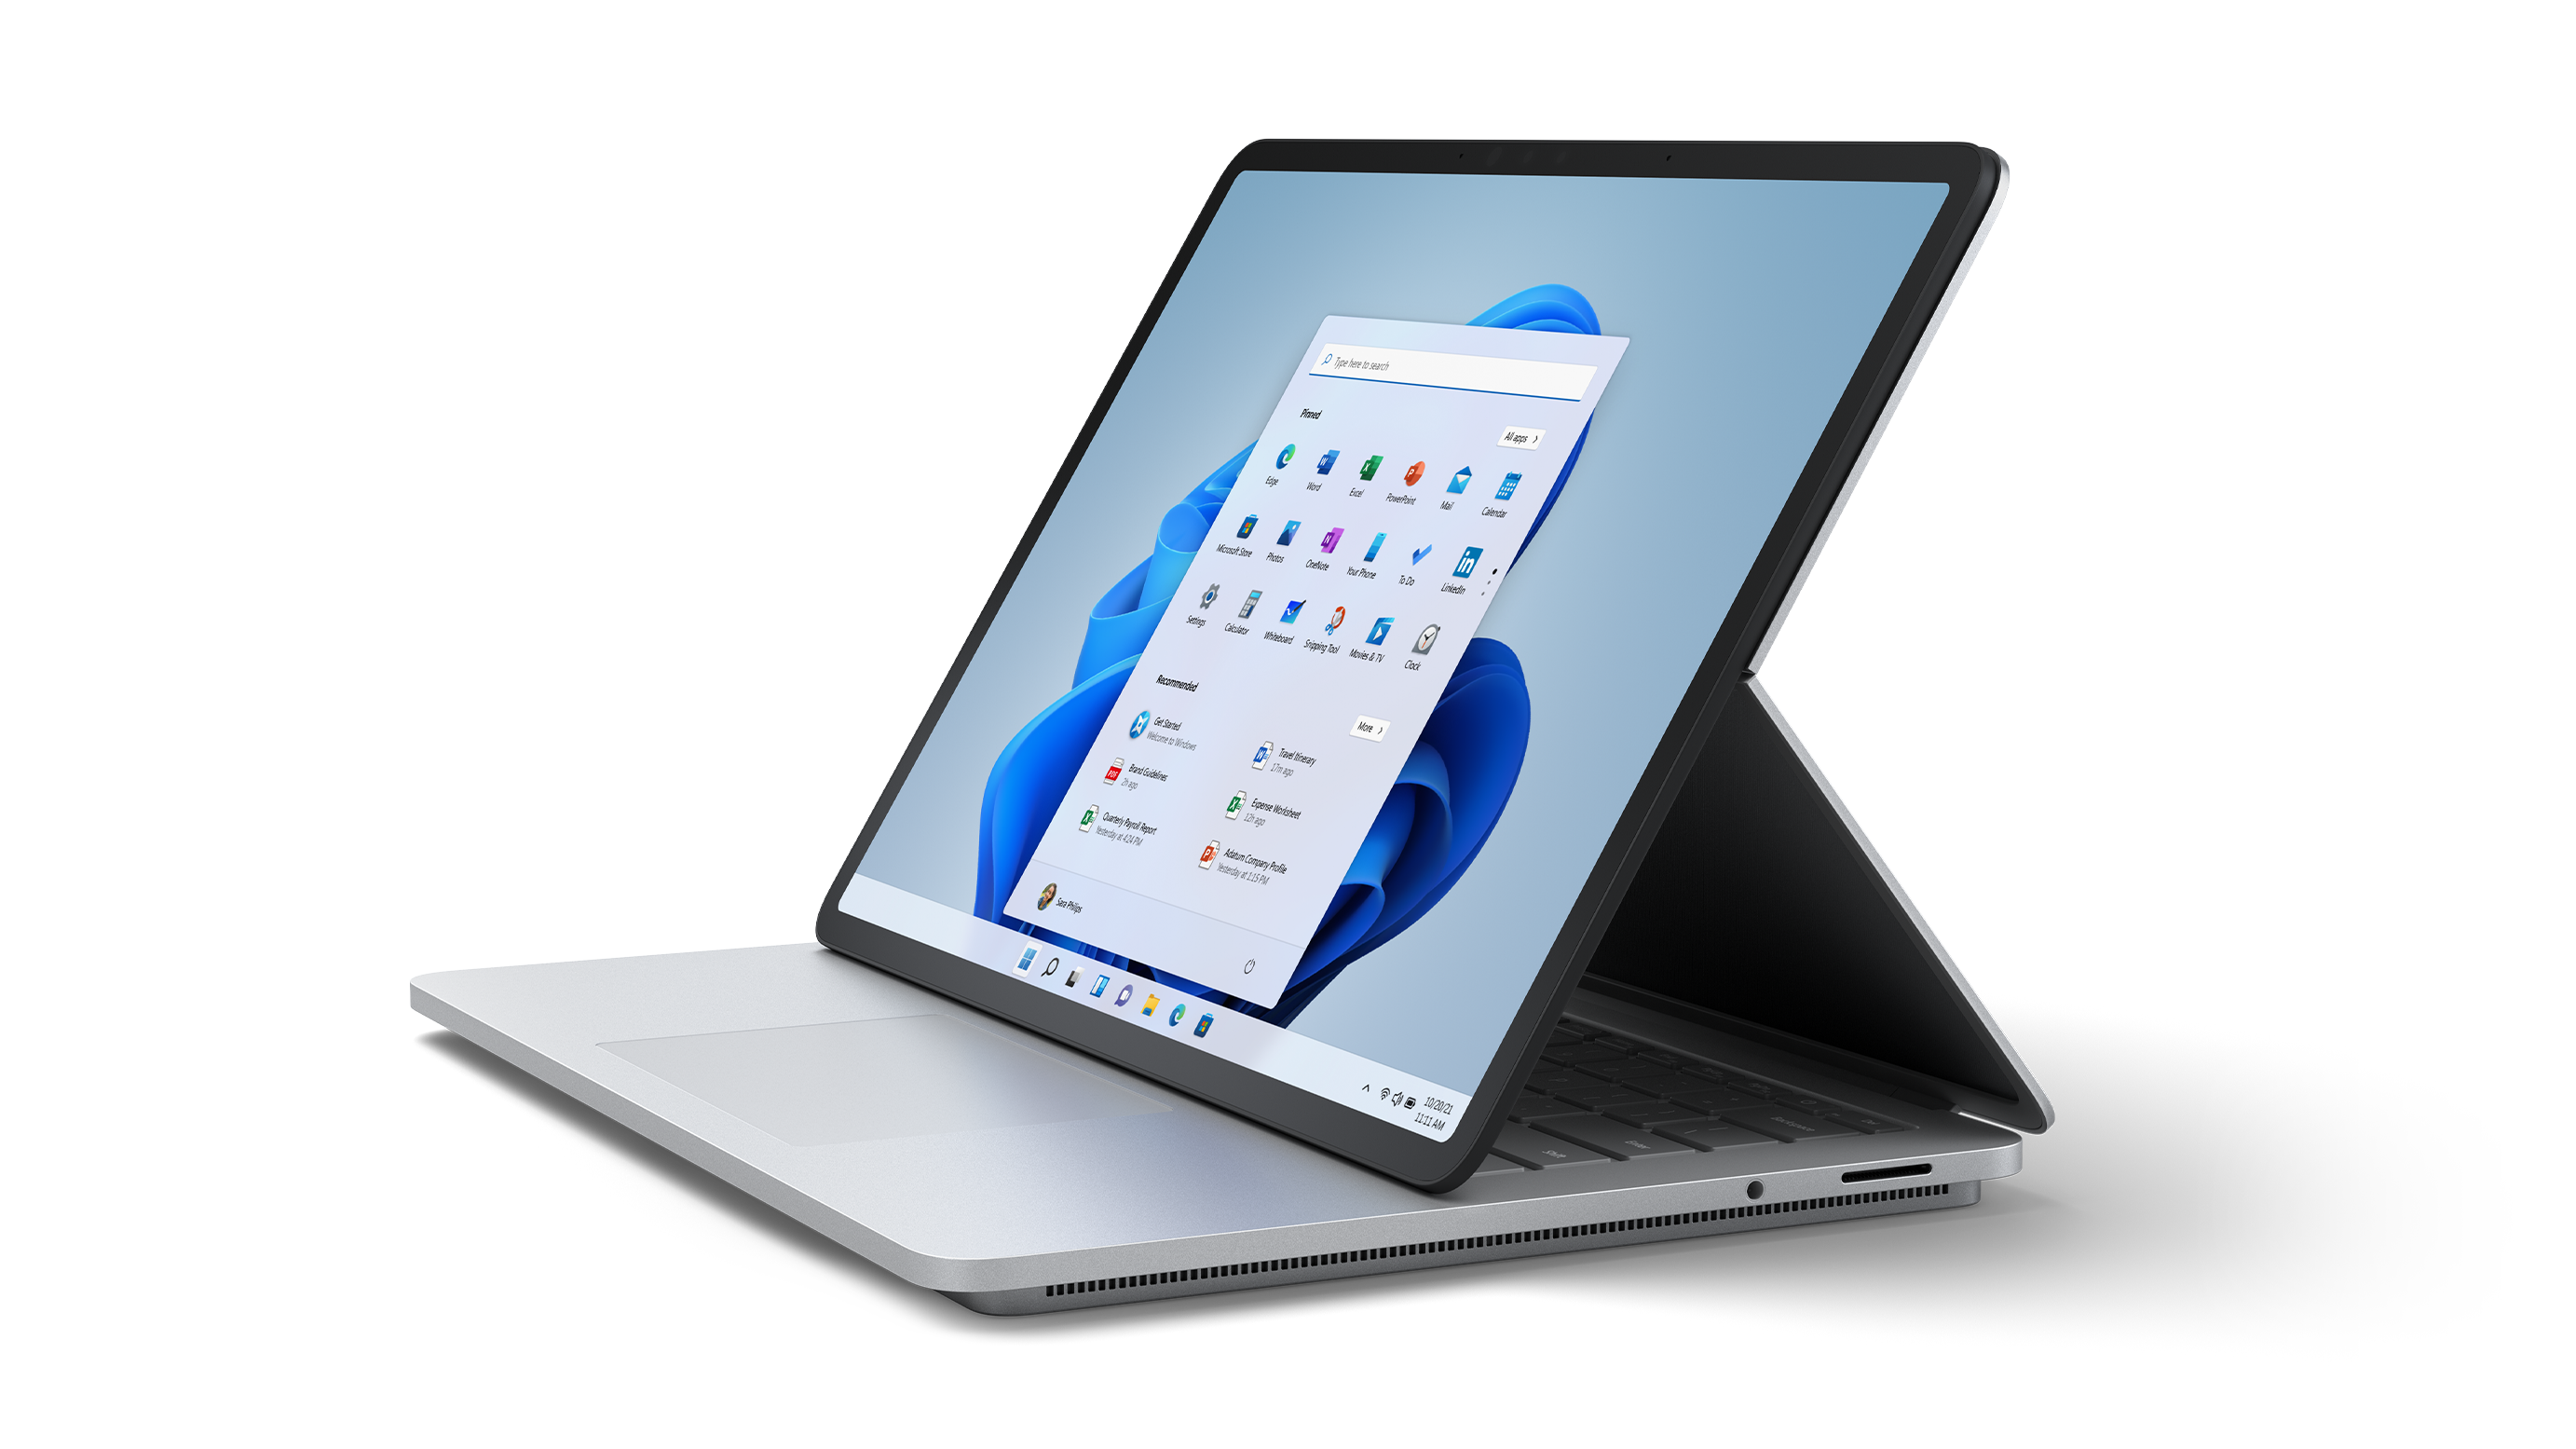
\includegraphics[width=8cm]{laptop.png}
              \caption{Notebook} \label{sistema}
       \end{center}
\end{figure}

\begin{figure}[H]
       \begin{center}
              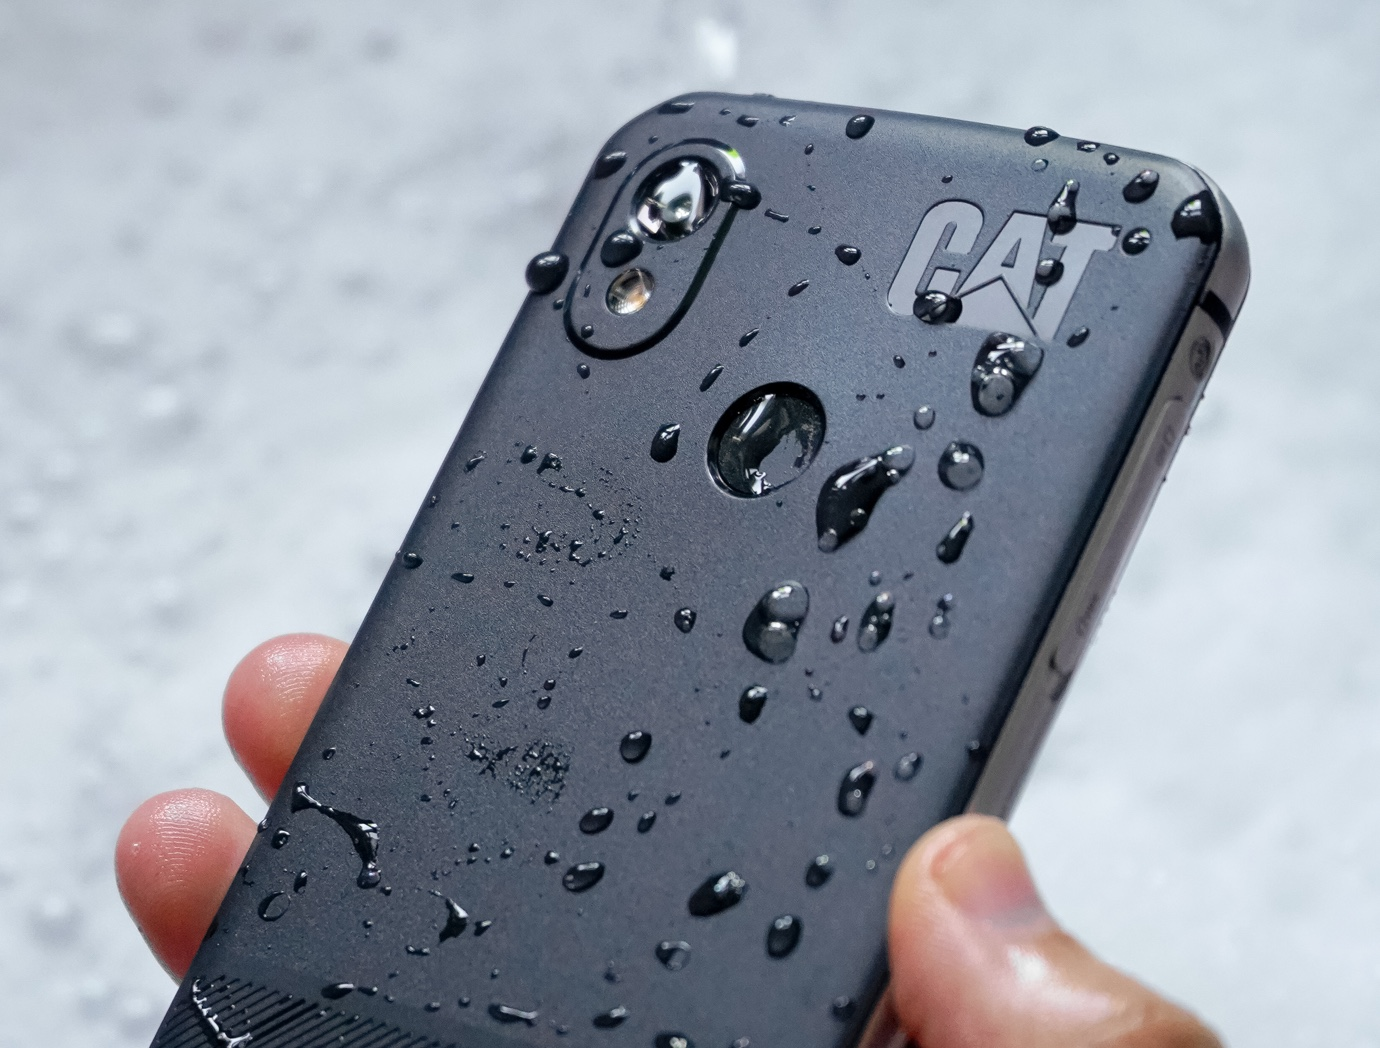
\includegraphics[width=8cm]{phone.jpg}
              \caption{Celular} \label{sistema}
       \end{center}
\end{figure}

\begin{figure}[H]
       \begin{center}
              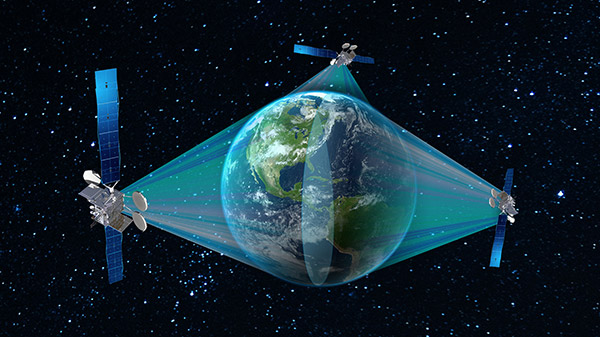
\includegraphics[width=8cm]{Satellite.jpg}
              \caption{Satellite} \label{sistema}
       \end{center}
\end{figure}

\begin{itemize}
       \item Smartphones;
        \item Aplicativo;
        \item Satélite artificial;
        \item Laptops.
        \end{itemize}

\subsection{Componente: Nuvem}

\begin{figure}[H]
       \begin{center}
              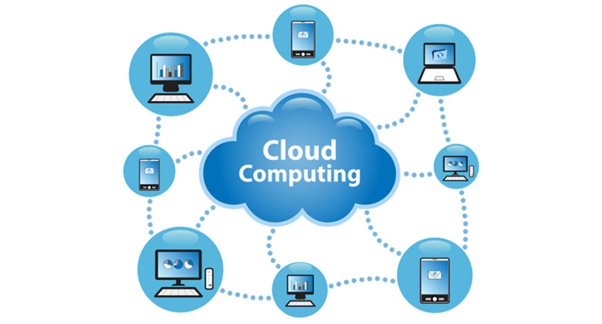
\includegraphics[width=8cm]{cloud.png}
              \caption{Cloud computing} \label{sistema}
       \end{center}
\end{figure}
\begin{figure}[H]
       \begin{center}
              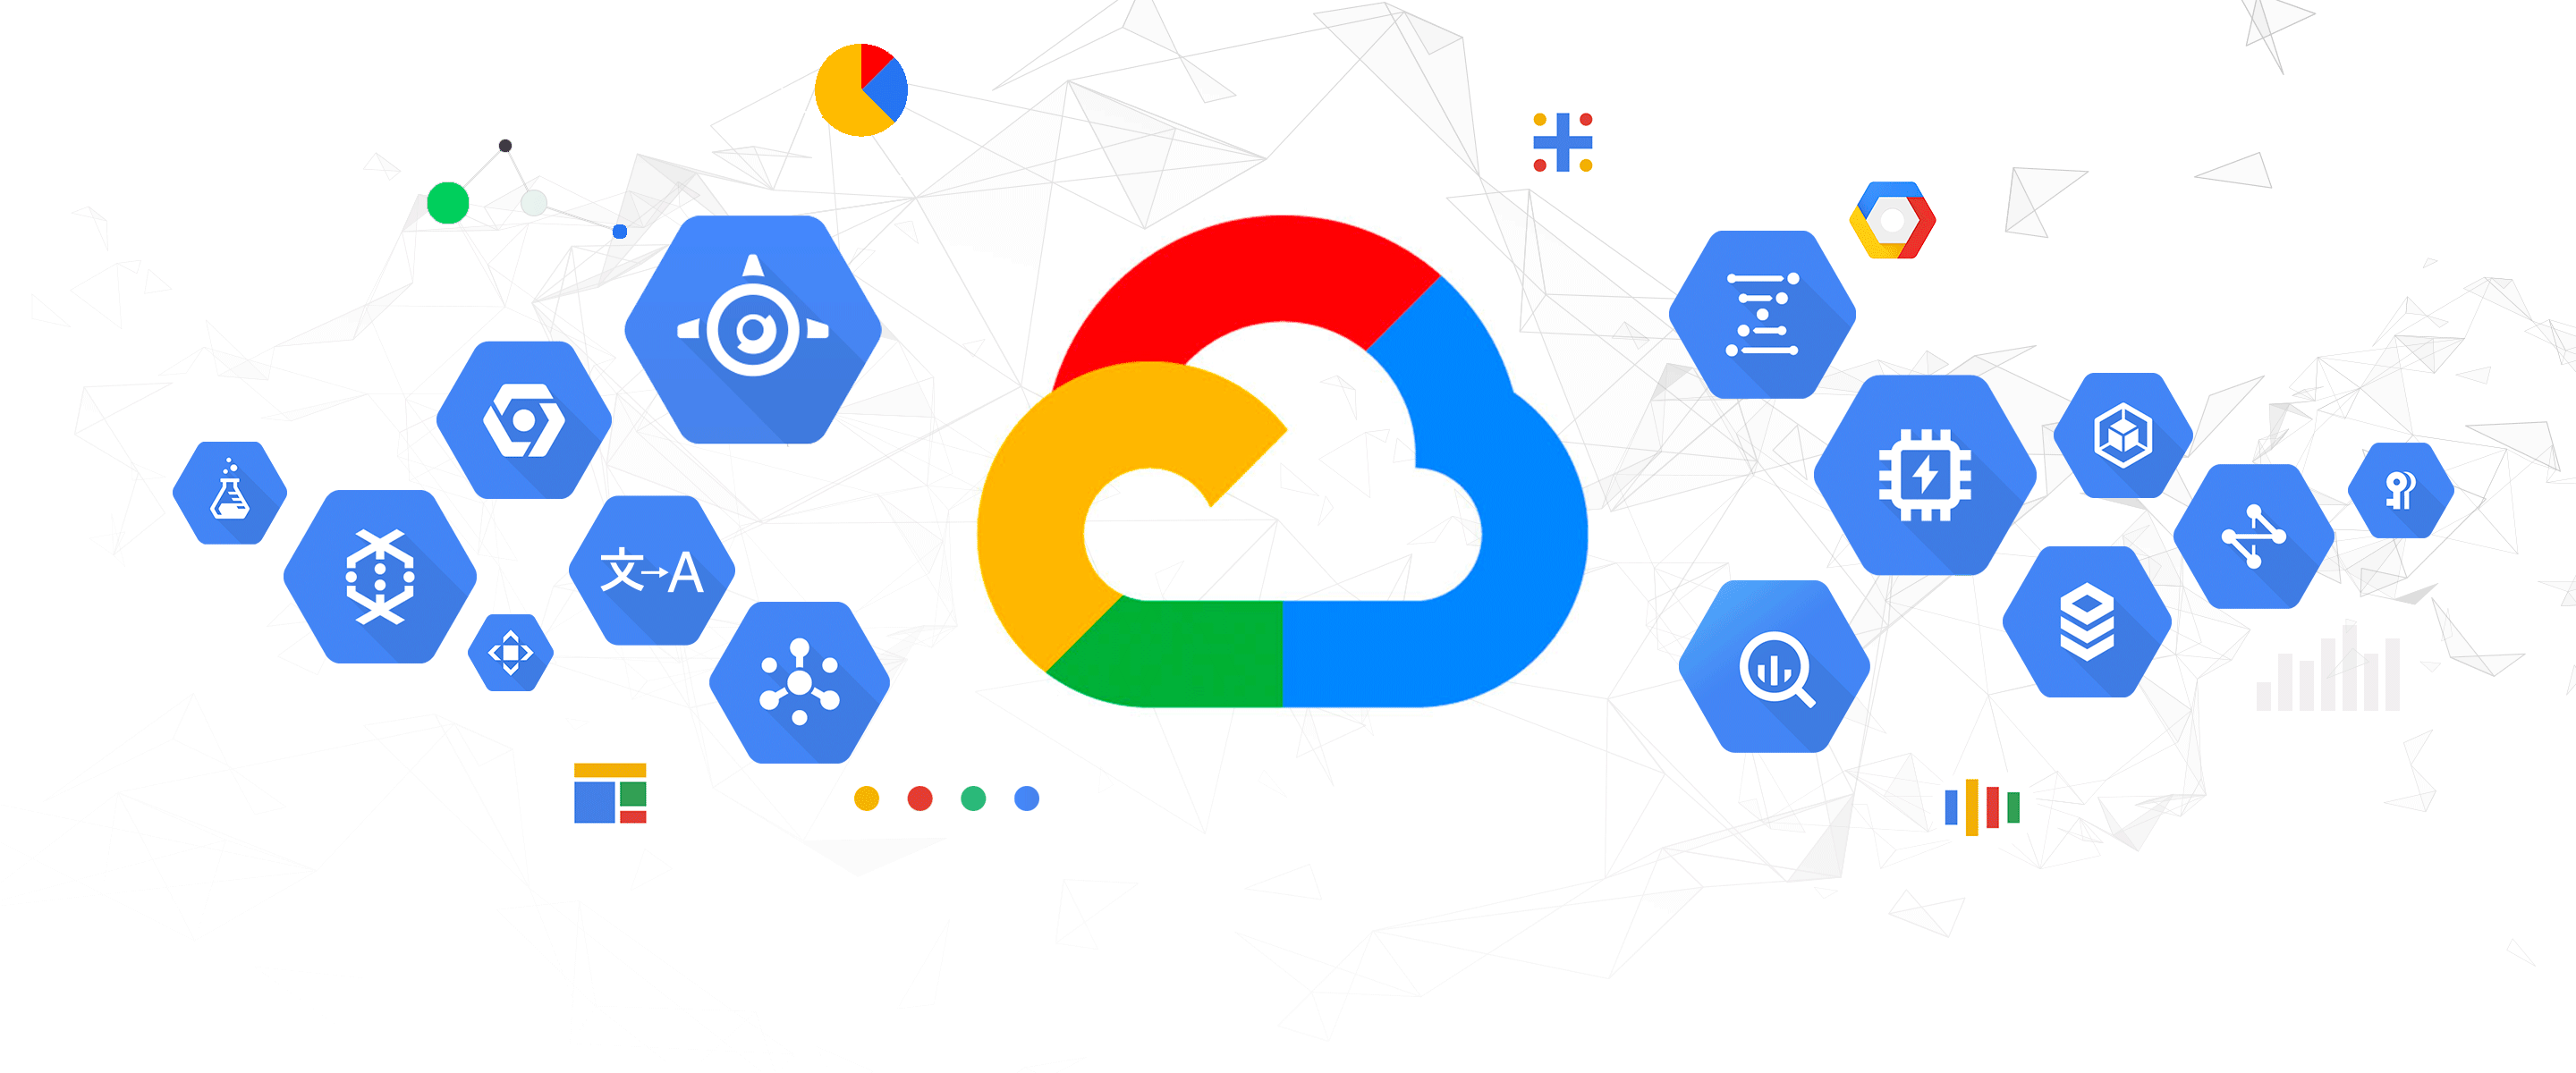
\includegraphics[width=8cm]{Google_Cloud_Covered.png}
              \caption{Cloud storage} \label{sistema}
       \end{center}
\end{figure}

\begin{itemize}
       \item Backup de dados;
       \item Hospedagem de aplicativo;
       \item Servidores;
        \subitem - Localização dos Veículos;
        \subitem - Conexão com usuários.

      \end{itemize}
